\documentclass[12pt,oneside]{report}

\usepackage[nottoc]{tocbibind}


\newcommand{\reporttitle}{Mixed Traffic Simulation for Autonomous Systems in Shared Spaces}
\newcommand{\reportauthor}{Frederik Tobias Hillier}
\newcommand{\reporttype}{Interim Report}
\newcommand{\cid}{01412520}

\newcommand{\supervisor}{Prof Y.K. Demiris}
\newcommand{\supervisorassistant}{Dr X. Zhang}
\newcommand{\secondmarker}{Prof D. Gunduz}


% include files that load packages and define macros
%%%%%%%%%%%%%%%%%%%%%%%%%%%%%%%%%%%%%%%%%
% University Assignment Title Page 
% LaTeX Template
% Version 1.0 (27/12/12)
%
% This template has been downloaded from:
% http://www.LaTeXTemplates.com
%
% Original author:
% WikiBooks (http://en.wikibooks.org/wiki/LaTeX/Title_Creation)
%
% License:
% CC BY-NC-SA 3.0 (http://creativecommons.org/licenses/by-nc-sa/3.0/)
% 
% Instructions for using this template:
% This title page is capable of being compiled as is. This is not useful for 
% including it in another document. To do this, you have two options: 
%
% 1) Copy/paste everything between \begin{document} and \end{document} 
% starting at \begin{titlepage} and paste this into another LaTeX file where you 
% want your title page.
% OR
% 2) Remove everything outside the \begin{titlepage} and \end{titlepage} and 
% move this file to the same directory as the LaTeX file you wish to add it to. 
% Then add \input{./title_page_1.tex} to your LaTeX file where you want your
% title page.
%
%----------------------------------------------------------------------------------------
%	PACKAGES AND OTHER DOCUMENT CONFIGURATIONS
%----------------------------------------------------------------------------------------
\usepackage{ifxetex}
\usepackage{textpos}
\usepackage{natbib}
\usepackage{kpfonts}
\usepackage[a4paper,hmargin=2.8cm,vmargin=2.0cm,includeheadfoot]{geometry}
\usepackage{ifxetex}
\usepackage{stackengine}
\usepackage{tabularx,longtable,multirow,subfigure,caption}%hangcaption
\usepackage{fncylab} %formatting of labels
\usepackage{fancyhdr}
\usepackage{color}
\usepackage[tight,ugly]{units}
\usepackage{url}
\usepackage{float}
\usepackage[english]{babel}
\usepackage{amsmath}
\usepackage{graphicx}
\usepackage[colorinlistoftodos]{todonotes}
\usepackage{dsfont}
\usepackage{epstopdf} % automatically replace .eps with .pdf in graphics
\usepackage{natbib}
\usepackage{backref}
\usepackage{array}
\usepackage{latexsym}
\usepackage{etoolbox}

\usepackage[english]{babel}
\usepackage[utf8x]{inputenc}

\usepackage{enumerate} % for numbering with [a)] format 

\bibpunct{[}{]}{,}{n}{,}{,}


%%% HEAD %%%
\fancyhf{}
\fancyhead[R]{\leftmark}
\usepackage{lastpage}
\fancyfoot[C]{\thepage} %/\pageref{LastPage}}



\ifxetex
\usepackage{fontspec}
\setmainfont[Scale=.8]{OpenDyslexic-Regular}
\else
\usepackage[pdftex,pagebackref,hypertexnames=false,colorlinks]{hyperref} % provide links in pdf
\hypersetup{pdftitle={},
  pdfsubject={}, 
  pdfauthor={\reportauthor},
  pdfkeywords={}, 
  pdfstartview=FitH,
  pdfpagemode={UseOutlines},% None, FullScreen, UseOutlines
  bookmarksnumbered=true, bookmarksopen=true, colorlinks,
    citecolor=black,%
    filecolor=black,%
    linkcolor=black,%
    urlcolor=black}
\usepackage[all]{hypcap}
\fi

\usepackage{tcolorbox}

% various theorems
\usepackage{ntheorem}
\theoremstyle{break}
\newtheorem{lemma}{Lemma}
\newtheorem{theorem}{Theorem}
\newtheorem{remark}{Remark}
\newtheorem{definition}{Definition}
\newtheorem{proof}{Proof}

% example-environment
\newenvironment{example}[1][]
{ 
\vspace{4mm}
\noindent\makebox[\linewidth]{\rule{\hsize}{1.5pt}}
\textbf{Example #1}\\
}
{ 
\noindent\newline\makebox[\linewidth]{\rule{\hsize}{1.0pt}}
}



%\renewcommand{\rmdefault}{pplx} % Palatino
% \renewcommand{\rmdefault}{put} % Utopia

\ifxetex
\else
\renewcommand*{\rmdefault}{bch} % Charter
\renewcommand*{\ttdefault}{cmtt} % Computer Modern Typewriter
%\renewcommand*{\rmdefault}{phv} % Helvetica
%\renewcommand*{\rmdefault}{iwona} % Avant Garde
\fi

\setlength{\parindent}{0em}  % indentation of paragraph

%\setlength{\headheight}{14.5pt}
\pagestyle{fancy}
%\fancyfoot[ER,OL]{\thepage}%Page no. in the left on
                                %odd pages and on right on even pages
%\fancyfoot[OC,EC]{\sffamily }
\renewcommand{\headrulewidth}{0.1pt}
\renewcommand{\footrulewidth}{0.1pt}
\captionsetup{margin=10pt,font=small,labelfont=bf}


%--- chapter heading

%\def\@makechapterhead#1{%
%  \vspace*{10\p@}%
%  {\parindent \z@ \raggedright %\sffamily
%        %{\Large \MakeUppercase{\@chapapp} \space \thechapter}
%        %\\
%        %\hrulefill
        %\par\nobreak
        %\vskip 10\p@
%    \interlinepenalty\@M
%    \Huge \bfseries 
%    \thechapter \space\space #1\par\nobreak
%    \vskip 30\p@
%  }}

%---chapter heading for \chapter*  
%\def\@makeschapterhead#1{%
%  \vspace*{10\p@}%
%  {\parindent \z@ \raggedright
%    \sffamily
%    \interlinepenalty\@M
%    \Huge \bfseries  
%    #1\par\nobreak
%    \vskip 30\p@
%  }}
 



% %%%%%%%%%%%%% boxit
\def\Beginboxit
   {\par
    \vbox\bgroup
	   \hrule
	   \hbox\bgroup
		  \vrule \kern1.2pt %
		  \vbox\bgroup\kern1.2pt
   }

\def\Endboxit{%
			      \kern1.2pt
		       \egroup
		  \kern1.2pt\vrule
		\egroup
	   \hrule
	 \egroup
   }	

\newenvironment{boxit}{\Beginboxit}{\Endboxit}
\newenvironment{boxit*}{\Beginboxit\hbox to\hsize{}}{\Endboxit}



\allowdisplaybreaks

\makeatletter
\newcounter{elimination@steps}
\newcolumntype{R}[1]{>{\raggedleft\arraybackslash$}p{#1}<{$}}
\def\elimination@num@rights{}
\def\elimination@num@variables{}
\def\elimination@col@width{}
\newenvironment{elimination}[4][0]
{
    \setcounter{elimination@steps}{0}
    \def\elimination@num@rights{#1}
    \def\elimination@num@variables{#2}
    \def\elimination@col@width{#3}
    \renewcommand{\arraystretch}{#4}
    \start@align\@ne\st@rredtrue\m@ne
}
{
    \endalign
    \ignorespacesafterend
}
\newcommand{\eliminationstep}[2]
{
    \ifnum\value{elimination@steps}>0\leadsto\quad\fi
    \left[
        \ifnum\elimination@num@rights>0
            \begin{array}
            {@{}*{\elimination@num@variables}{R{\elimination@col@width}}
            |@{}*{\elimination@num@rights}{R{\elimination@col@width}}}
        \else
            \begin{array}
            {@{}*{\elimination@num@variables}{R{\elimination@col@width}}}
        \fi
            #1
        \end{array}
    \right]
    & 
    \begin{array}{l}
        #2
    \end{array}
    &%                                    moved second & here
    \addtocounter{elimination@steps}{1}
}
\makeatother

%% Fast macro for column vectors
\makeatletter  
\def\colvec#1{\expandafter\colvec@i#1,,,,,,,,,\@nil}
\def\colvec@i#1,#2,#3,#4,#5,#6,#7,#8,#9\@nil{% 
  \ifx$#2$ \begin{bmatrix}#1\end{bmatrix} \else
    \ifx$#3$ \begin{bmatrix}#1\\#2\end{bmatrix} \else
      \ifx$#4$ \begin{bmatrix}#1\\#2\\#3\end{bmatrix}\else
        \ifx$#5$ \begin{bmatrix}#1\\#2\\#3\\#4\end{bmatrix}\else
          \ifx$#6$ \begin{bmatrix}#1\\#2\\#3\\#4\\#5\end{bmatrix}\else
            \ifx$#7$ \begin{bmatrix}#1\\#2\\#3\\#4\\#5\\#6\end{bmatrix}\else
              \ifx$#8$ \begin{bmatrix}#1\\#2\\#3\\#4\\#5\\#6\\#7\end{bmatrix}\else
                 \PackageError{Column Vector}{The vector you tried to write is too big, use bmatrix instead}{Try using the bmatrix environment}
              \fi
            \fi
          \fi
        \fi
      \fi
    \fi
  \fi 
}  
\makeatother

\robustify{\colvec}

%%% Local Variables: 
%%% mode: latex
%%% TeX-master: "notes"
%%% End: 
 % various packages needed for maths etc.
% quick way of adding a figure
\newcommand{\fig}[3]{
 \begin{center}
 \scalebox{#3}{\includegraphics[#2]{#1}}
 \end{center}
}

%\newcommand*{\point}[1]{\vec{\mkern0mu#1}}
\newcommand{\ci}[0]{\perp\!\!\!\!\!\perp} % conditional independence
\newcommand{\point}[1]{{#1}} % points 
\renewcommand{\vec}[1]{{\boldsymbol{{#1}}}} % vector
\newcommand{\mat}[1]{{\boldsymbol{{#1}}}} % matrix
\newcommand{\R}[0]{\mathds{R}} % real numbers
\newcommand{\Z}[0]{\mathds{Z}} % integers
\newcommand{\N}[0]{\mathds{N}} % natural numbers
\newcommand{\nat}[0]{\mathds{N}} % natural numbers
\newcommand{\Q}[0]{\mathds{Q}} % rational numbers
\ifxetex
\newcommand{\C}[0]{\mathds{C}} % complex numbers
\else
\newcommand{\C}[0]{\mathds{C}} % complex numbers
\fi
\newcommand{\tr}[0]{\text{tr}} % trace
\renewcommand{\d}[0]{\mathrm{d}} % total derivative
\newcommand{\inv}{^{-1}} % inverse
\newcommand{\id}{\mathrm{id}} % identity mapping
\renewcommand{\dim}{\mathrm{dim}} % dimension
\newcommand{\rank}[0]{\mathrm{rk}} % rank
\newcommand{\determ}[1]{\mathrm{det}(#1)} % determinant
\newcommand{\scp}[2]{\langle #1 , #2 \rangle}
\newcommand{\kernel}[0]{\mathrm{ker}} % kernel/nullspace
\newcommand{\img}[0]{\mathrm{Im}} % image
\newcommand{\idx}[1]{{(#1)}}
\DeclareMathOperator*{\diag}{diag}
\newcommand{\E}{\mathds{E}} % expectation
\newcommand{\var}{\mathds{V}} % variance
\newcommand{\gauss}[2]{\mathcal{N}\big(#1,\,#2\big)} % gaussian distribution N(.,.)
\newcommand{\gaussx}[3]{\mathcal{N}\big(#1\,|\,#2,\,#3\big)} % gaussian distribution N(.|.,.)
\newcommand{\gaussBig}[2]{\mathcal{N}\left(#1,\,#2\right)} % see above, but with brackets that adjust to the height of the arguments
\newcommand{\gaussxBig}[3]{\mathcal{N}\left(#1\,|\,#2,\,#3\right)} % see above, but with brackets that adjust to the height of the arguments
\DeclareMathOperator{\cov}{Cov} % covariance (matrix) 
\ifxetex
\renewcommand{\T}[0]{^\top} % transpose
\else
\newcommand{\T}[0]{^\top}
\fi
% matrix determinant
\newcommand{\matdet}[1]{
\left|
\begin{matrix}
#1
\end{matrix}
\right|
}



%%% various color definitions
\definecolor{darkgreen}{rgb}{0,0.6,0}

\newcommand{\blue}[1]{{\color{blue}#1}}
\newcommand{\red}[1]{{\color{red}#1}}
\newcommand{\green}[1]{{\color{darkgreen}#1}}
\newcommand{\orange}[1]{{\color{orange}#1}}
\newcommand{\magenta}[1]{{\color{magenta}#1}}
\newcommand{\cyan}[1]{{\color{cyan}#1}}


% redefine emph
\renewcommand{\emph}[1]{\blue{\bf{#1}}}

% place a colored box around a character
\gdef\colchar#1#2{%
  \tikz[baseline]{%
  \node[anchor=base,inner sep=2pt,outer sep=0pt,fill = #2!20] {#1};
    }%
}%
 % short-hand notation and macros


%%%%%%%%%%%%%%%%%%%%%%%%%%%%

\begin{document}
% front page
\begin{titlepage}

\newcommand{\HRule}{\rule{\linewidth}{0.5mm}} % Defines a new command for the horizontal lines, change thickness here


%----------------------------------------------------------------------------------------
%	LOGO SECTION
%----------------------------------------------------------------------------------------

% 
\includegraphics[width = 4cm]{./figures/imperial}\\[0.5cm] 

\begin{center} % Center remainder of the page

%----------------------------------------------------------------------------------------
%	HEADING SECTIONS
%----------------------------------------------------------------------------------------
\textsc{\LARGE \reporttype}\\[1.5cm] 
\textsc{\Large Imperial College London}\\[0.5cm] 
\textsc{\large Department of Electronic and Electrical Engineering}\\[0.5cm] 
%----------------------------------------------------------------------------------------
%	TITLE SECTION
%----------------------------------------------------------------------------------------

\HRule \\[0.4cm]
{ \huge \bfseries \reporttitle}\\ % Title of your document
\HRule \\[1.5cm]
\end{center}
%----------------------------------------------------------------------------------------
%	AUTHOR SECTION
%----------------------------------------------------------------------------------------

%\begin{minipage}{0.4\hsize}
\begin{flushleft} \large
\textit{Author:}\\
\reportauthor~(CID: \cid) % Your name
\end{flushleft}
\vspace{1cm}

\begin{flushleft} \large
\textit{Supervisor:}\\
\supervisor %~(CID: \cid) % Your name
\end{flushleft}
\vspace{1cm}

\begin{flushleft} \large
\textit{Second Marker:}\\
\secondmarker % ~(CID: \cid) % Your name
\end{flushleft}
\vspace{2cm}
\makeatletter
Date: \@date 

\vfill % Fill the rest of the page with whitespace



\makeatother


\end{titlepage}



\tableofcontents
\newpage

%%%%%%%%%%%%%%%%%%%%%%%%%%%% Main document
\chapter{Introduction}
\newcommand\tab[1][1cm]{\hspace*{#1}}

\section{Report Outline}
This is the interim report for my master's thesis titled "Mixed Traffic Simulation for Autonomous Systems in Shared Spaces". The report aims to present the initial background research and early implementation results \cite{studentGuideline}. The report will contain the following sections as suggested in the project guide:
\\ \tab The \emph{Introduction} chapter will establish the project outline and the expected deliverables. The chapter will also describe the context of the underlying problem the project will try to resolve.
\\ \tab The \emph{Background} chapter will first introduce the technical tools and theory needed to understand the project. This will include looking at what a game engine is, as well as briefly looking at the two major game engines used by most simulators. Thereafter comes an analysis of the simulators that have been studied with a conclusion for which simulator was chosen for this project. 
\\ \tab The \emph{Implementation} chapter will describe what work has been done in regards to the chosen simulator. The chapter will also contain an evaluation plan for how the project deliverables will be evaluated. In addition, the chapter will show the estimated timeline and possible extensions. 
\\ \tab And finally the \emph{Ethical, Legal and Safety Considerations} chapter which will look if there are any ethical legal or safety concerns both in regards to the project as is, but also briefly with potential extensions.

\pagebreak
\section{Project Specification} \label{ProjectSpec}
\subsection{Objectives} \label{Objectives}
The objectives of the project are: 
\begin{itemize}
    \item Survey the current state of the art in vehicle and mobile robot simulation and evaluate current simulators (e.g. CARLA, CrowdSim3D, Gazebo), list and understand the underlying simulation methodologies (e.g. types of physics engine), and understand and document their advantages and disadvantages, particularly in terms of their sensing and control abilities.
    \item Select the most suitable current simulator that offers potential for incorporating mixed traffic (for example, cars, mobile robots/wheelchairs, humans, cyclists, and so on), and 3D environments/maps.
    \item Create a process for incorporating and controlling agent models with an API (e.g. ability to add control abilities to the human model, for example to move their bodies, and to grasp objects).
    \item Add sensors to the simulated agents (e.g. cameras, LIDARS) and a perception API, where simulation users can obtain sensing data from the simulator, for example what can the agents “see” in their environment.
\end{itemize}
(Source: Project Specification as written by Prof. Y. K. Demiris)
\\~\\~\\
Features that want to have in our simulator: 
\begin{itemize}
\item Be able to place agents
\item Control the agents' behavior
\item Access to what the agent sees as well as body movement
\item Looking to plot a path for pedestrians
\item Able to drive off the road, e.g. on the pavement and interact with pedestrians
\item Want to easily create custom maps which are not whole worlds
\item Does not need to handle a large number of pedestrians and vehicles
\item Not looking to be able to navigate indoors
\item Animation and realistic car movement is not important
\end{itemize}
(Source: After discussion in the supervisor meetings, 22/10 and 10/11)
\subsection{Deliverables}
The main deliverables for this project will be:
\begin{itemize}
    \item An analysis of available simulators with a conclusion for which one to use for the project.
    \item A simulator with the ability to easily add additional models and simulate mixed traffic.
    \item A simulator with the incorporated sensing and controlling APIs.
    \item Documentation for how to use the two above points.
\end{itemize}
If time allows for it there could be a possibility of extending the project, but that is still to be determined (Section~\ref{Extensions}) 
\section{Context}
For the last decade there has been a lot of talk about self-driving cars and other autonomous systems \cite{markoff_2010}. Back in 2010 most autonomous systems were only driven on closed circuits, but today there are a variety of car manufacturers offering autopilot on their cars. In 2021 Tesla have announced that all new cars they produce will have the hardware needed for full automation in almost all circumstances \cite{teslaSelf}. 
\\~\\ 
Compared to 2010 when the autonomous cars were mainly driven on closed tracks, the modern-day self-driving car will have to operate alongside other cars on the road as well as alongside pedestrians.  This is where the concept of shared spaces comes in. The autonomous system must now take other entities into account when making decisions. 
\\~\\ 
As other entities’ actions can be complex to forecast, machine learning models can be used to predict the outcome of a situation more easily. These models can be trained much faster on a simulator than in real life. This is because the simulator can simulate many different configurations at once. An autonomous system in real life cannot replicate the exact same environment, whilst this can easily be done in a simulation.  
\\~\\ 
Another advantage of using a simulator is that you can learn from doing mistakes, whilst in real life, mistakes can be both dangerous and costly. In the simulator, the autonomous system can learn without the risk of colliding with an actual person or damaging other cars. Running simulations is therefore a good way to train the machine learning model much faster and safer than on a real road.  
\\~\\ 
The autonomous system does not have to be a vehicle, but anything that can artificial control itself. These could for example be mobile robots/wheelchairs or artificial controlled humans and cyclists. 
\\~\\ 
This project will consist of three main parts. The first one being to research available simulators (Section~\ref{BackgroundLit}). This will be necessary to get a good starting point for the project. Working on an existing simulator that is too complex would mean that it would take too long to get basic features working. Whilst working on a simulator that does not have enough features will mean that too much time will be spent implementing something that another simulator will already have implemented. Exactly what these features are will be clarified in the Project Specification chapter (Chapter~\ref{ProjectSpec}). 
The second part will be to implement the missing features from the simulator that we selected to work on.
And the last part will be to determine what to do next with the simulator after the missing features have been implemented. This is still open-ended, but some of the potential use cases will be discussed in the Implementation section (Section~\ref{FuturePlanning}).
\\~\\ 
The product generated from this project could be used for a variety of different use cases. Firstly it could be used to test the software for an autonomous system. Testing it in a simulator would be much faster than trying to check for corner cases in real life. Another example would be to train a machine learning model. The simulator will aim to be a diverse tool to accommodate a variety of needs. 



\chapter{Background}

\section{Background Theory}
\subsection{Physics Engines}

\subsubsection{Open Dynamics Engine (ODE)}
\subsubsection{PhysX}


\subsection{Rendering Engines}  % Maybe not needed
\subsubsection{Open Graphics Rendering Engine (OGRE)}

\subsection{Game Engines}
The purpose of a game engine is to work as a fundamental back-end for most video games and simulators. A game engine is a software tool which allows interactive digital content to be made using a framework which easily allows the user to run it on different platforms such as computers, smartphones and consoles \cite{GameEngine_UnityGame_book}. Game engines are complex and consists of many components such as a physics engine, a rendering engine and other interactive tools to help the creator. They give the creator the freedom to control everything from lighting and audio to animation and character behavior in their game.
\\~\\
There exists many different game engines, but the two main ones that are currently in existence is Unity and Unreal Engine. These allow beginners to easily create their first games, as well as professional companies creating their games for millions of users \cite{GamesMadeInUnity, GamesMadeInUnrealEngine}.

\subsubsection{Unity}
Unity is currently the most commonly used game engine and over 2.5 million registered developers \cite{Unity_arnia_software}. Unity is developed by Unity Technologies and was first released June 2005.  Originally Unity was Over 60\% of augmented- and virtual reality games are created using Unity  \cite{GameEngine_UnityGame_book}. 
\\~\\
Unity is free for personal and educational projects. To create the game, Unity allows a lot of features using the GUI, but for full freedom the creator would need to program in C\#. Unity however provide lots of resources to learn C\#. Unity also combines with Visual Studio where the intellisense can help with recommending functions to use as well as spot errors\footnote{\url{https://docs.microsoft.com/en-us/visualstudio/gamedev/unity/get-started/getting-started-with-visual-studio-tools-for-unity}}.

\subsubsection{Unreal Engine}
Unreal Engine is a fast growing game engine and is created by Epic Games \cite{UnrealEngine_Book}. The first version of Unreal Engine was released in 1998, but Unreal Engine 4 (UE4), which was released September 2014, is their latest game engine. They have however announced that they will release Unreal Engine 5 (UE5) at the end of 2021 \cite{UE5}. 
\\~\\
UE4 has a variety of different use cases as well as games. TV broadcastes such as Sky Sports and BBC are using Unreal Engine for their graphical match analysis \cite{UnrealEngine_LiveBroadcast}. Professional architects are also using the product to illustrate their creations \cite{UnrealEngine_Automative}.   
\\~\\
Unreal Engine 4 is free for personal use and business making less than \$1 million in gross revenue \cite{UE5}. The code for UE4 is available on GitHub\footnote{\url{https://github.com/EpicGames/UnrealEngine}} (For access to the repository you would need to sign up for an Epic Games account\footnote{\url{https://www.unrealengine.com/en-US/ue4-on-github}}). UE4 allows two different ways for users to program their games. Either by using C++, which links with Visual Studio\footnote{\url{https://docs.unrealengine.com/en-US/ProductionPipelines/DevelopmentSetup/VisualStudioSetup/index.html}}, or by using blueprints as illustrated in Figure~\ref{UnrealEngineBlueprint}. Blueprints allows the creator for most of the freedom code gives them, but in an easier drag and drop layout.
\\~\\
The majority of the simulators that will be looked at later use Unreal Engine as their game engine. 

\begin{figure}[H] 
    \centering
    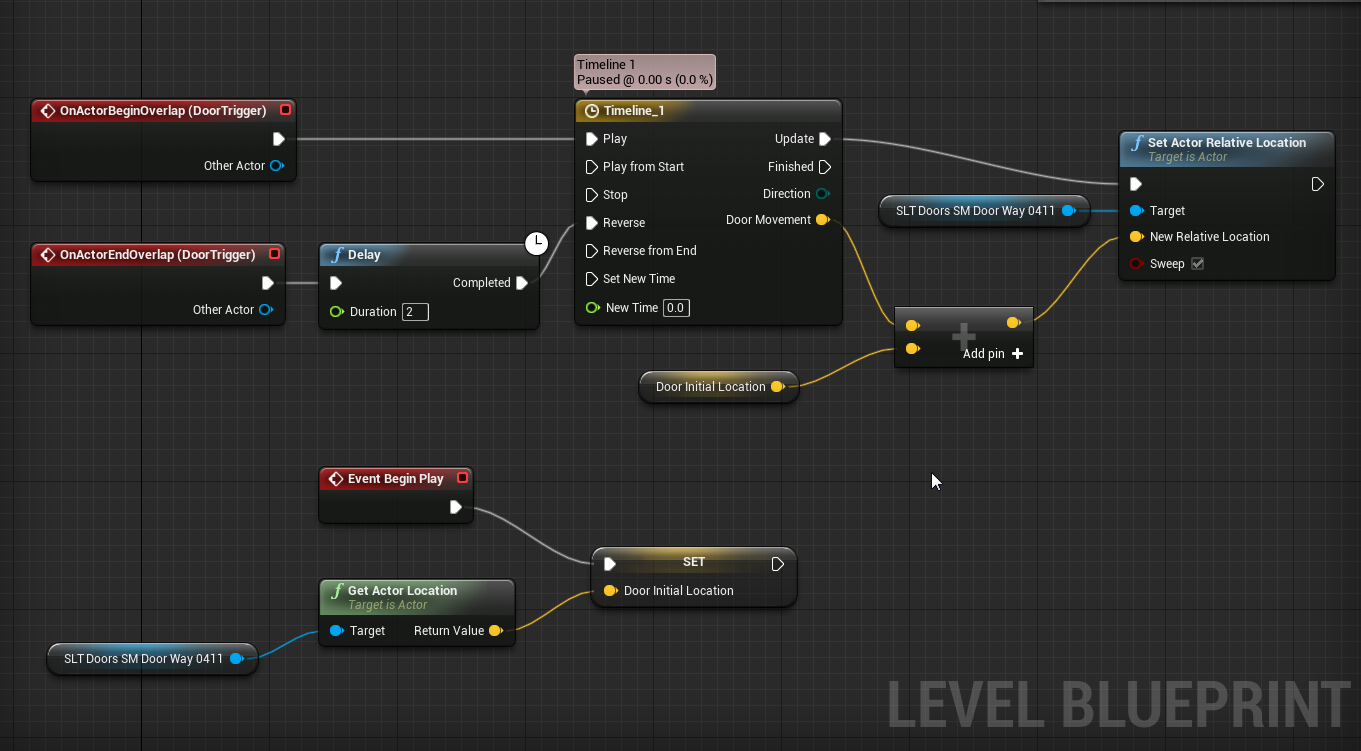
\includegraphics[width=0.5\textwidth]{OtherImages/UEBlueprint.png}
    \caption{Source: \url{https://docs.unrealengine.com/en-US/ProgrammingAndScripting/Blueprints/UserGuide/Timelines/Examples/OpeningDoors/index.html}}    \label{UnrealEngineBlueprint}

\end{figure}


\subsection{Traffic Simulators}


\section{Analysis of Relevant Literature} \label{BackgroundLit}
In this section we will look at a large variety of different simulators, to determine which one best suits our purpose. We will be looking at which operating system and game engine the simulator uses, whether or not it is open source, and the pros and cons of each simulator. We will be particularly looking at the simulators sensing abilities, ability to add additional entities, map customisability, available APIs, and how user-friendly the simulator is. Aspects of the simulator which is not as important as how realistic the simulator physics is, and how visually good looking it is. These are criteria formed by the project specification (Section~\ref{ProjectSpec})
\\~\\
The purpose of this was to get a good understanding of the different simulators currently in existence. The aim was to find 3-4 simulators that would be worth looking closer at.

%%%%%%%% 4DV-Sim %%%%%%%%%%
\subsection{4DV-Sim}
\textbf{Description:} 4DV-Sim\footnote{Website: \url{https://www.4d-virtualiz.com/en/automotive-simulator}} is a simulator that is designed to emulate the hardware and sensors in autonomous systems. This is a professional product and has a variety of use cases from simulating farming to the military.

\textbf{Open Source:} No

\textbf{Operating System:} Linux

\textbf{Game Engine:} Non, but it does use PhysX for the physics engine

\textbf{Pros:} The simulator has a lot of available APIs. The simulator also comes with a configurable GUI to set up the simulation environment how you would like it. Also, as it is professionally made, it looks very good.   

\textbf{Cons:} It is not designed to train machine learning implementations on the simulator, but rather emulate a current hardware setup. Also, as it is not open source, it will not be something that we could modify or expand upon to suit our purposes. 

\textbf{Conclusion:} As 4DV-Sim is not an open-source product it is not something that we can use for this project. It is however interesting to see that simulators like this are needed not just for research purposes, but for customers who want to try out their hardware setup in an emulated environment.


\begin{figure}[H]
    \centering
    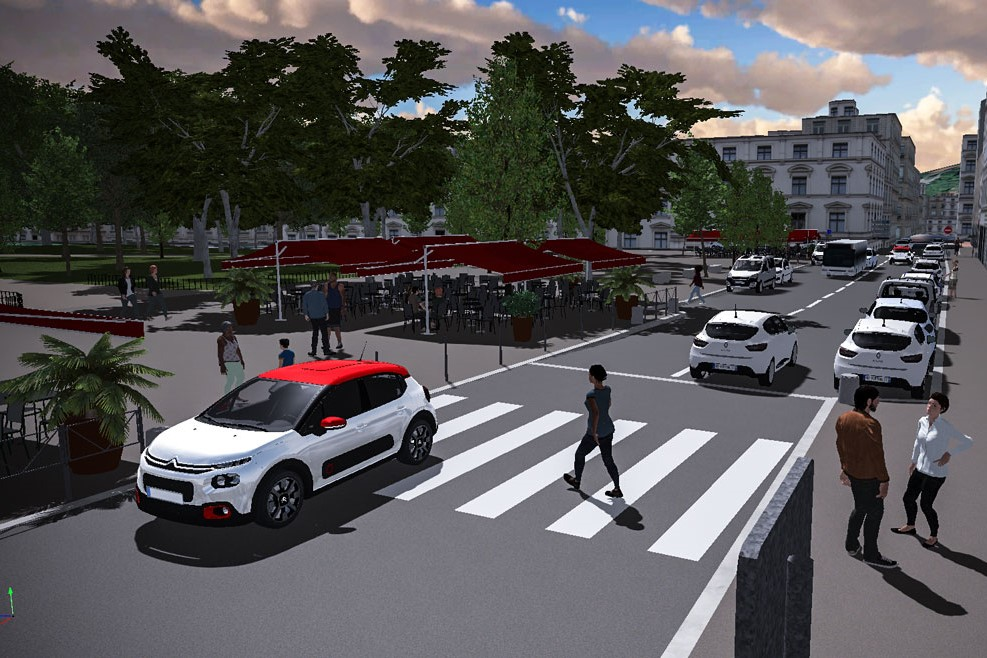
\includegraphics[width=0.5\textwidth]{Simulators/4DV-Sim.jpg}
    \caption{Source: \url{https://www.4d-virtualiz.com/en/automotive-simulator}}
\end{figure}

%%%%%%%% AirSIM %%%%%%%%%%
\subsection{AirSim}
\textbf{Description:} AirSim\footnote{Website: \url{https://microsoft.github.io/AirSim}} is a simulator for cars and drones. It is open-source and works as a plugin for unreal engine, which means the simulator can be used with any environment which has been modeled inside the game engine. According to their website \cite{AirSim_Website}, the goal of the simulator is to create a platform for AI research to experiment with deep learning, computer vision, and reinforcement learning algorithms for autonomous systems. 

\textbf{Open Source:} Yes

\textbf{Operating System:} Any operating system

\textbf{Game Engine:} Primarily Unreal Engine, but it also offers a prototype version in Unity

\textbf{Pros:} Offers a large range of existing APIs. The simulator also has an active community on both discord and Github. It also gives the option to add drones. It is also designed to train machine learning algorithms on it.

\textbf{Cons:} The simulator is not as realistic as other simulators. The vehicle physics is not as good as some of the other simulators, for example the handling and collisions. Also, currently, there are no pedestrians in the game. 

\textbf{Conclusion:} AirSim is worth looking closer into. As it is built using a game engine it should not be too hard to add the missing features, like for example adding and controlling pedestrians. Also, realistic vehicle physics was determined not to be an important factor for this project. 

\begin{figure}[H]
    \centering
    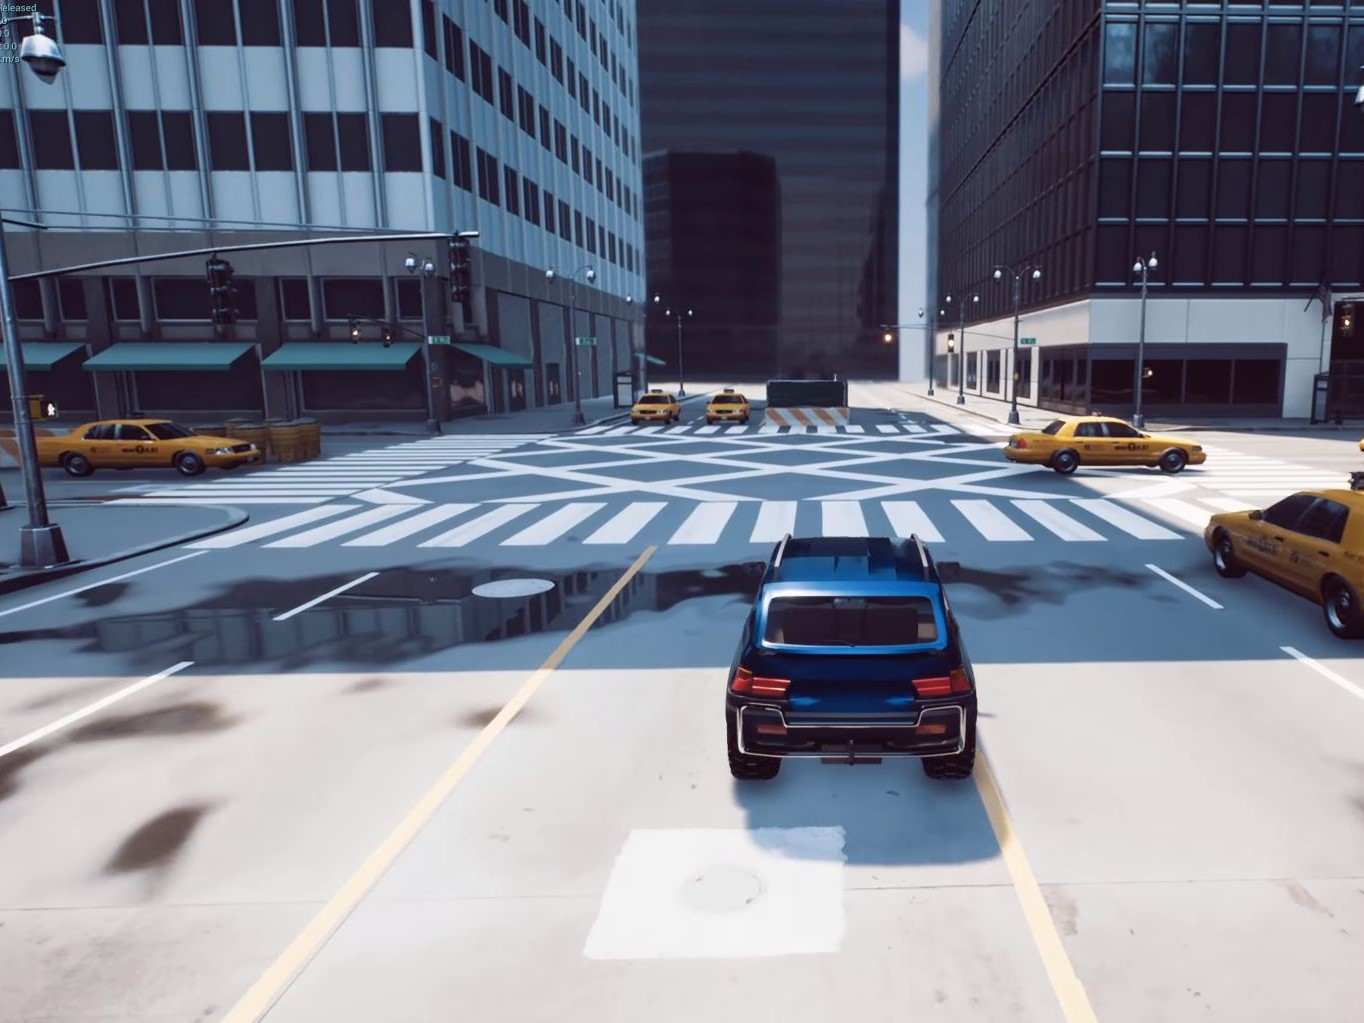
\includegraphics[width=0.5\textwidth]{Simulators/AirSim.JPG}
    \caption{Source: \url{https://microsoft.github.io/AirSim}}
\end{figure}

%%%%%%%% Apollo %%%%%%%%%%
\subsection{Apollo} \label{Apollo}
\textbf{Description:} Apollo is a simulator that is designed to emulate the hardware in autonomous vehicles so that it can be trained for machine learning algorithms. According to their website \cite{Apollo_Website}, Apollo is a flexible architecture that accelerates the development and testing of autonomous vehicles.

\textbf{Open Source:} Yes

\textbf{Operating System:} Any system that can run Docker

\textbf{Game Engine:} Unity

\textbf{Pros:} Accurately models the vehicle physics to help improve the machine learning algorithms accuracy. The simulator is also actively being worked on by a large community.  

\textbf{Cons:} It looks like quite a complex simulator, and it does therefore not seem like it will be easy to modify. The product is really specific towards training autonomous vehicles. 

\textbf{Conclusion:} Due to the complexity of this simulator, it does not look like something that we could build upon for this project. 

\begin{figure}[H]
    \centering
    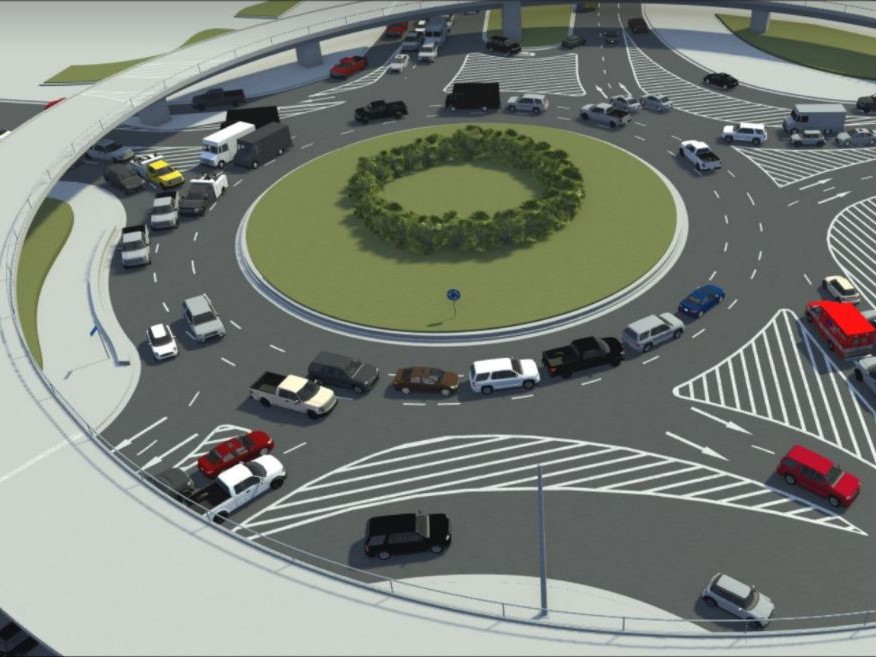
\includegraphics[width=0.5\textwidth]{Simulators/Apollo.JPG}
    \caption{Source: Slide deck from Apollo Game Engine Based Simulation Talk at GDC 2019 - \url{https://bit.ly/2VSzwlF}}
\end{figure}

%%%%%%%% Autoware %%%%%%%%%%
\subsection{Autoware} \label{Autoware}
\textbf{Description:} Autoware is an open-source software for autonomous vehicles. It comes with a large variety of APIs  \cite{Autoware_doc_Website}. Autoware is however not a simulator but can be used on a simulated vehicle to make it autonomous.

\textbf{Open Source:} Yes

\textbf{Operating System:} Robot Operating System (ROS)

\textbf{Game Engine:} Na

\textbf{Pros:} As it runs on ROS it can easily be adapted to work on a real autonomous vehicle.

\textbf{Cons:} Currently it only works with a specific car model and sensor set up. The software also seems quite complex, and combining it with a simulator will probably be quite challenging.

\textbf{Conclusion:} As this is not a simulator this is not something that we can use for this project. We will see with the LGSVL simulator (\ref{LGSVL_Simulator}), this software can be used alongside a simulator to model the autonomous system. 


%%%%%%%% Carla %%%%%%%%%%
\subsection{Carla}
\textbf{Description:} Carla is an open-source simulator for developing autonomous vehicles. It contains a variety of APIs and is actively being developed. Carla is also designed for training machine learning algorithms. 

\textbf{Open Source:} Yes

\textbf{Operating System:} Primarily Linux, but also Windows

\textbf{Game Engine:} Unreal Engine

\textbf{Pros:} Has a lot of features already implemented, such as sensors, vehicle API, and the ability to add new objects. Active community. Well documented and lots of information online. 

\textbf{Cons:} Difficult to add new and custom maps. Vehicle handling is not as realistic as some of the other simulators.

\textbf{Conclusion:} Carla is worth looking into further as it has most of the features that we are looking for.


\begin{figure}[H]
    \centering
    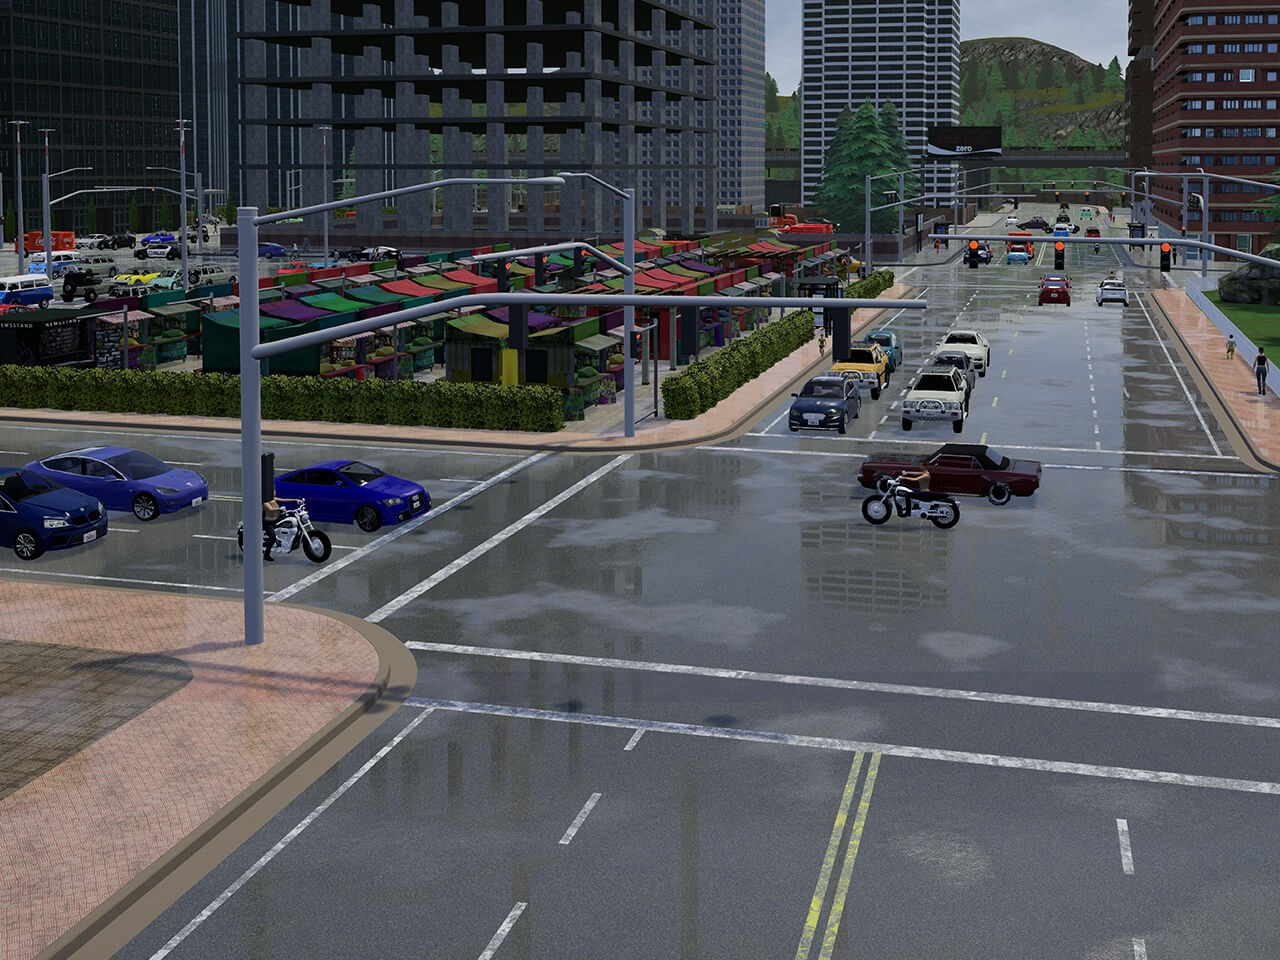
\includegraphics[width=0.5\textwidth]{Simulators/Carla.JPG}
    \caption{Source: \url{https://www.unrealengine.com/en-US/spotlights/carla-democratizes-autonomous-vehicle-r-d-with-free-open-source-simulator}}
\end{figure}


%%%%%%%% CrowdSim3D %%%%%%%%%%
\subsection{CrowdSim3D}
\textbf{Description:} CrowdSim3D is primarily a simulator for modeling large crowds, but can also be used for vehicle traffic. 

\textbf{Open Source:} No (£180)

\textbf{Operating System:} Any operating system

\textbf{Game Engine:} Not specified

\textbf{Pros:} Has the ability to control several pedestrians and vehicles in a shared space.

\textbf{Cons:} Does not look to be designed for machine learning algorithms. Difficult to add new models. Also, as it is not open source it will not be possible to customise the product. 

\textbf{Conclusion:} CrowdSim3D is not worth considering as we cannot adapt the product as it is not open source. 

\begin{figure}[H]
    \centering
    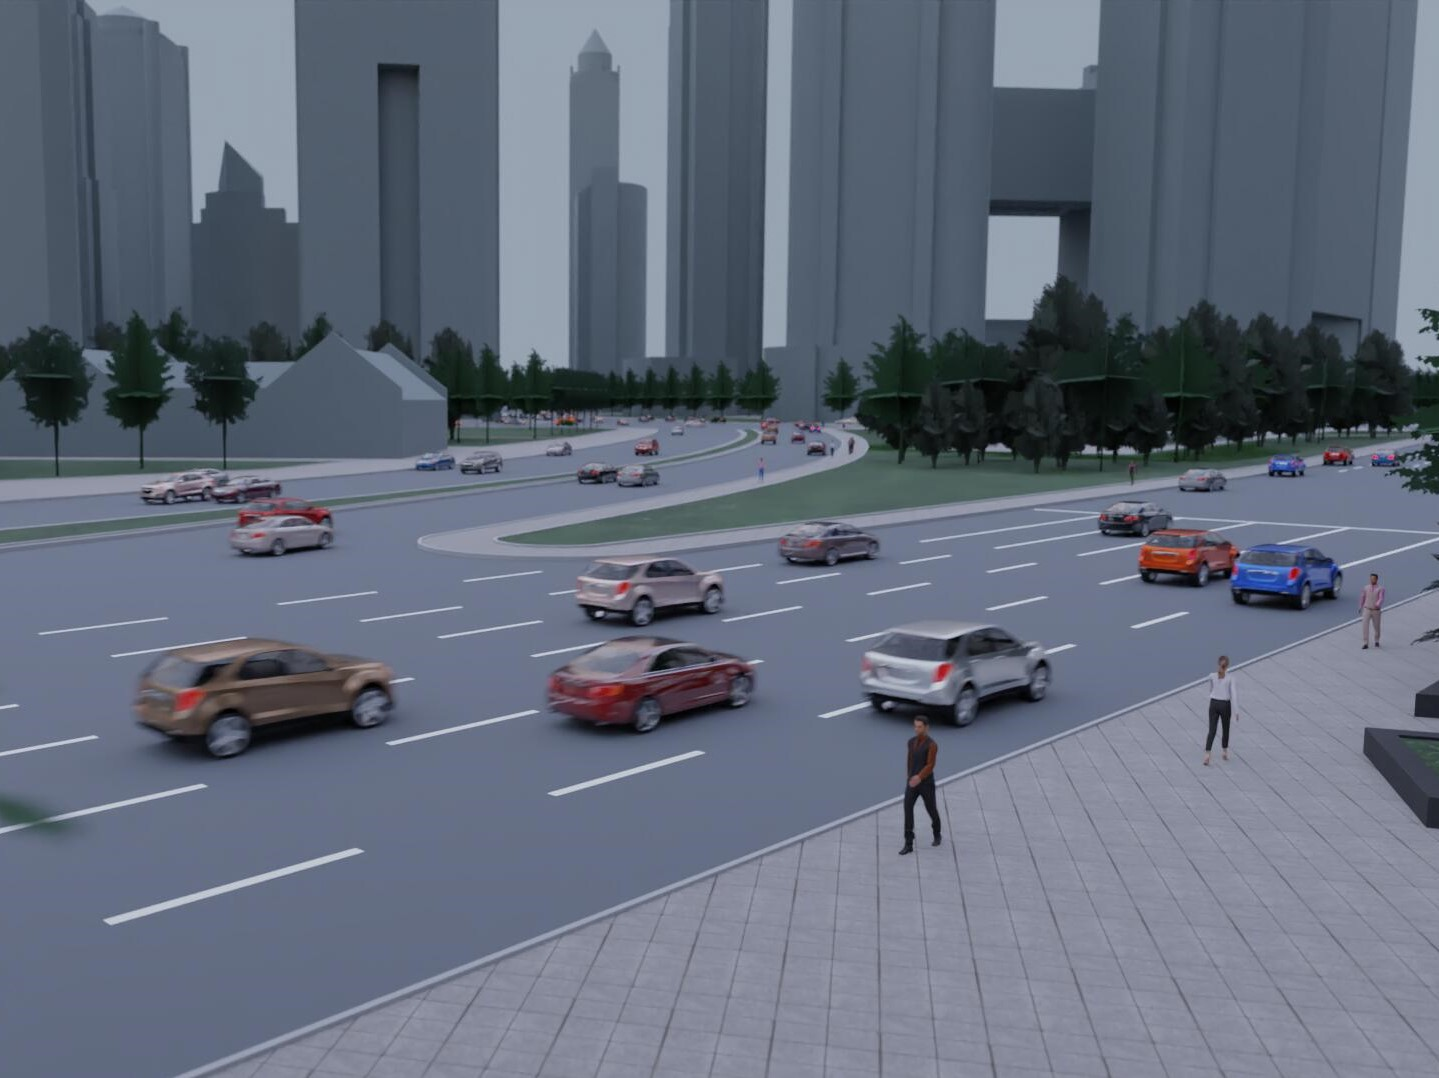
\includegraphics[width=0.5\textwidth]{Simulators/CrowdSim.JPG}
    \caption{Source: \url{https://crowdsim3d.com}}
\end{figure}


%%%%%%%% Deep Drive %%%%%%%%%%
\subsection{Deep Drive}
\textbf{Description:} Deep Drive \cite{DeepDrive_Website} is an open-source simulator aimed to train neural networks for self-driving cars. They also provide you with a large data set to train your autonomous vehicle on. 

\textbf{Open Source:} yes

\textbf{Operating System:} Any operating system

\textbf{Game Engine:} Unreal Engine

\textbf{Pros:} Is able to handle a variety of different sensors and vehicle setups. It also has an active community and a leader board where you can compare your trained neural network against other developers. 

\textbf{Cons:} Currently there are three maps available, but it is not easy to add your own maps. Also, it is not designed to be customised. Currently, there are no pedestrians and no APIs.

\textbf{Conclusion:} Deep Drive is not a simulator that is worth looking at as it is not designed to be customised. It also lacks most of the features we are looking for. 

\begin{figure}[H]
    \centering
    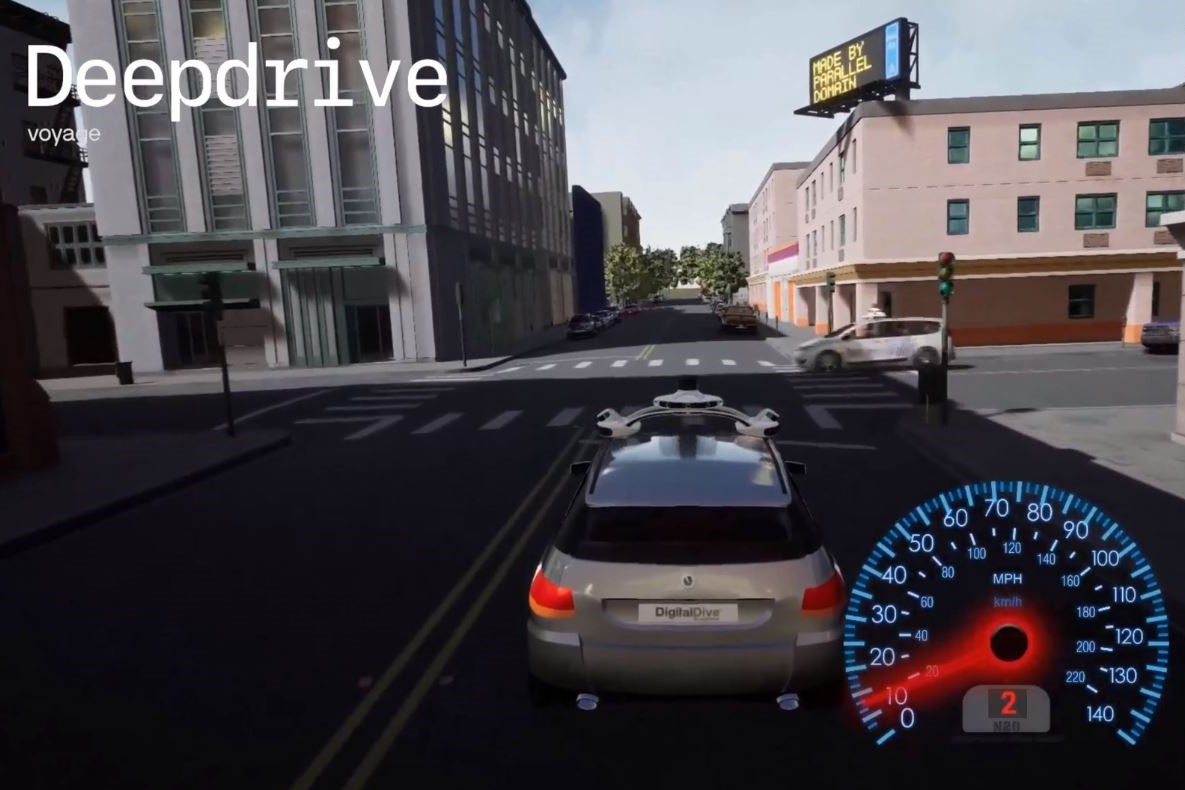
\includegraphics[width=0.5\textwidth]{Simulators/DeepDrive.JPG}
    \caption{Source: \url{https://deepdrive.voyage.auto}}
\end{figure}

%%%%%%%% Donkey Car Simulator %%%%%%%%%%
\subsection{Donkey Car Simulator}
\textbf{Description:} Donkey Car Simulator is a simulator for the Donkey Car. The car itself costs roughly £200 and can be ordered online, or you can download the schematics for free. The simulator can be used to train a neural network in Python which can then run on your car. 

\textbf{Open Source:} Yes

\textbf{Operating System:} Any operating system

\textbf{Game Engine:} Unity

\textbf{Pros:} Easy to use

\textbf{Cons:} Not what we are looking for as it is only used to train a real toy car.

\textbf{Conclusion:} Donkey Car is an interesting project to read about as it is a fun kit that introduces people to autonomous cars. However, it is not what we are looking for for this project as the simulator is not customisable and there is only one vehicle. 


\begin{figure}[H]
    \centering
    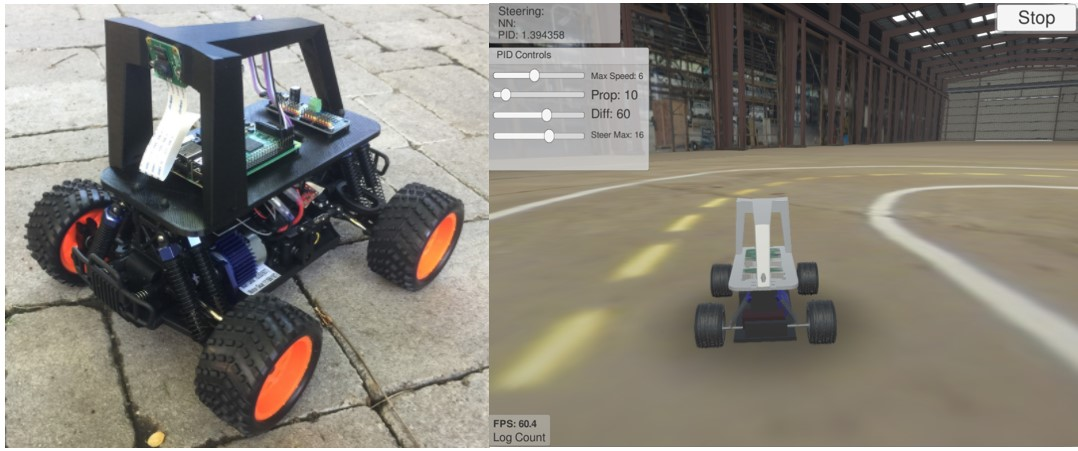
\includegraphics[width=0.5\textwidth]{Simulators/DonkeySim.jpg}
    \caption{Source: \url{https://docs.donkeycar.com}}
\end{figure}

%%%%%%%% Gazebo %%%%%%%%%%
\subsection{Gazebo}
\textbf{Description:}

\textbf{Open Source:} Yes

\textbf{Operating System:} Any operating system

\textbf{Game Engine:} ODE, Bullet, Simbody, DART

\textbf{Pros:}

\textbf{Cons:}

\textbf{Conclusion:} 


\begin{figure}[H]
    \centering
    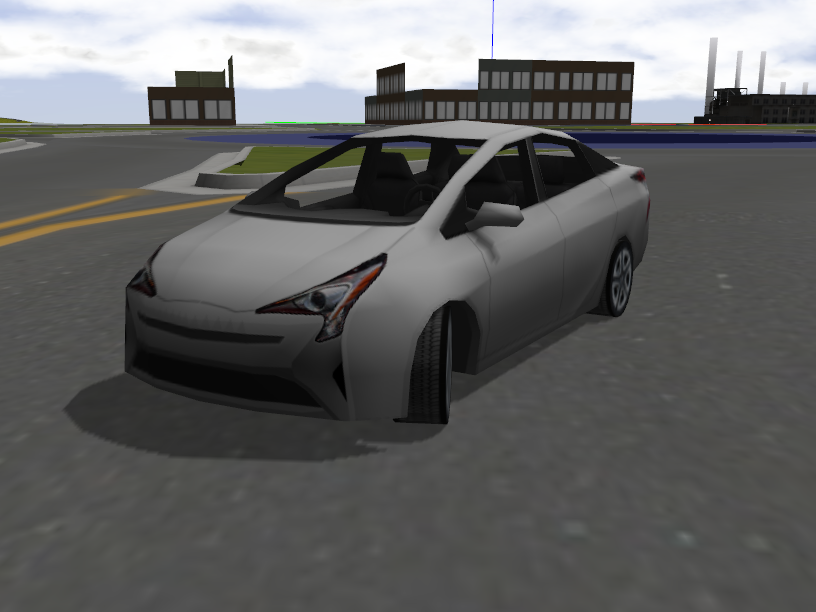
\includegraphics[width=0.5\textwidth]{Simulators/gazebo.png}
    \caption{Source: \url{http://gazebosim.org/blog/vehicle\%20simulation}}
\end{figure}


%%%%%%%% LPZRobots %%%%%%%%%%
\subsection{LPZRobots}
\textbf{Description:} LPZRobots is a robotics simulator created by the Robotics Group for Self-Organisation of Control at the University of Leipzig in Germany \cite{LPZRobots_Website, LPZRobots_book}. The simulator aims to have an open environment to simulate the robot's physics. 

\textbf{Open Source:} Yes

\textbf{Operating System:} Primarily Linux, but now also supports Linux

\textbf{Game Engine:} ODE

\textbf{Pros:} Free to add any kind of robot.

\textbf{Cons:} The code has not been updated since 2018 and the last release was in 2016. Unlike other simulators, this one does not seem to have an active community. 

\textbf{Conclusion:} As the development of the LPZRobots simulator has been inactive for several years, makes it not worth considering. The simulator also lacks most of the features we are looking for. 

\begin{figure}[H]
    \centering
    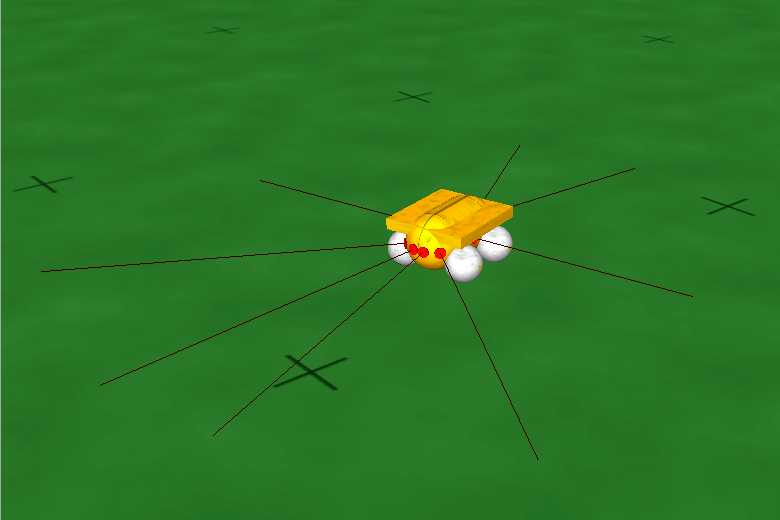
\includegraphics[width=0.5\textwidth]{Simulators/LPZRobots.png}
    \caption{Source: \url{https://itp.uni-frankfurt.de/~gros/StudentProjects/Robots\_2016\_ObstacleAvoidance}}
\end{figure}


%%%%%%%% LGSVL Simulator %%%%%%%%%%
\subsection{LGSVL Simulator} \label{LGSVL_Simulator}
\textbf{Description:} LGSVL is a simulator created by the Advanced Platform Lab at the LG Electronics America R\&D Center \cite{LGSVL_Web}. The simulator combines the vehicle from Autoware (Section~\ref{Autoware}) with Apollo (Section~\ref{Apollo}) which emulates the hardware. The LGSVL has lots of available APIs such as cameras, LiDAR, RADAR, and GPS. Some environmental parameters can also be changed such as the map, weather, and pedestrians.
% Uses Apollo and Autoware

\textbf{Open Source:} Yes

\textbf{Operating System:} Windows 10

\textbf{Game Engine:} A variety due to its complexness, but both Unreal Engine and Unity.

\textbf{Pros:} Has most of the features we are looking for.

\textbf{Cons:} Relies on a lot of different components. The codebase is therefore large and complex and it looks difficult to add our own features such as our own entity.

\textbf{Conclusion:} The LGSVL Simulator would probably not work for us as it seems too complex.

\begin{figure}[H]
    \centering
    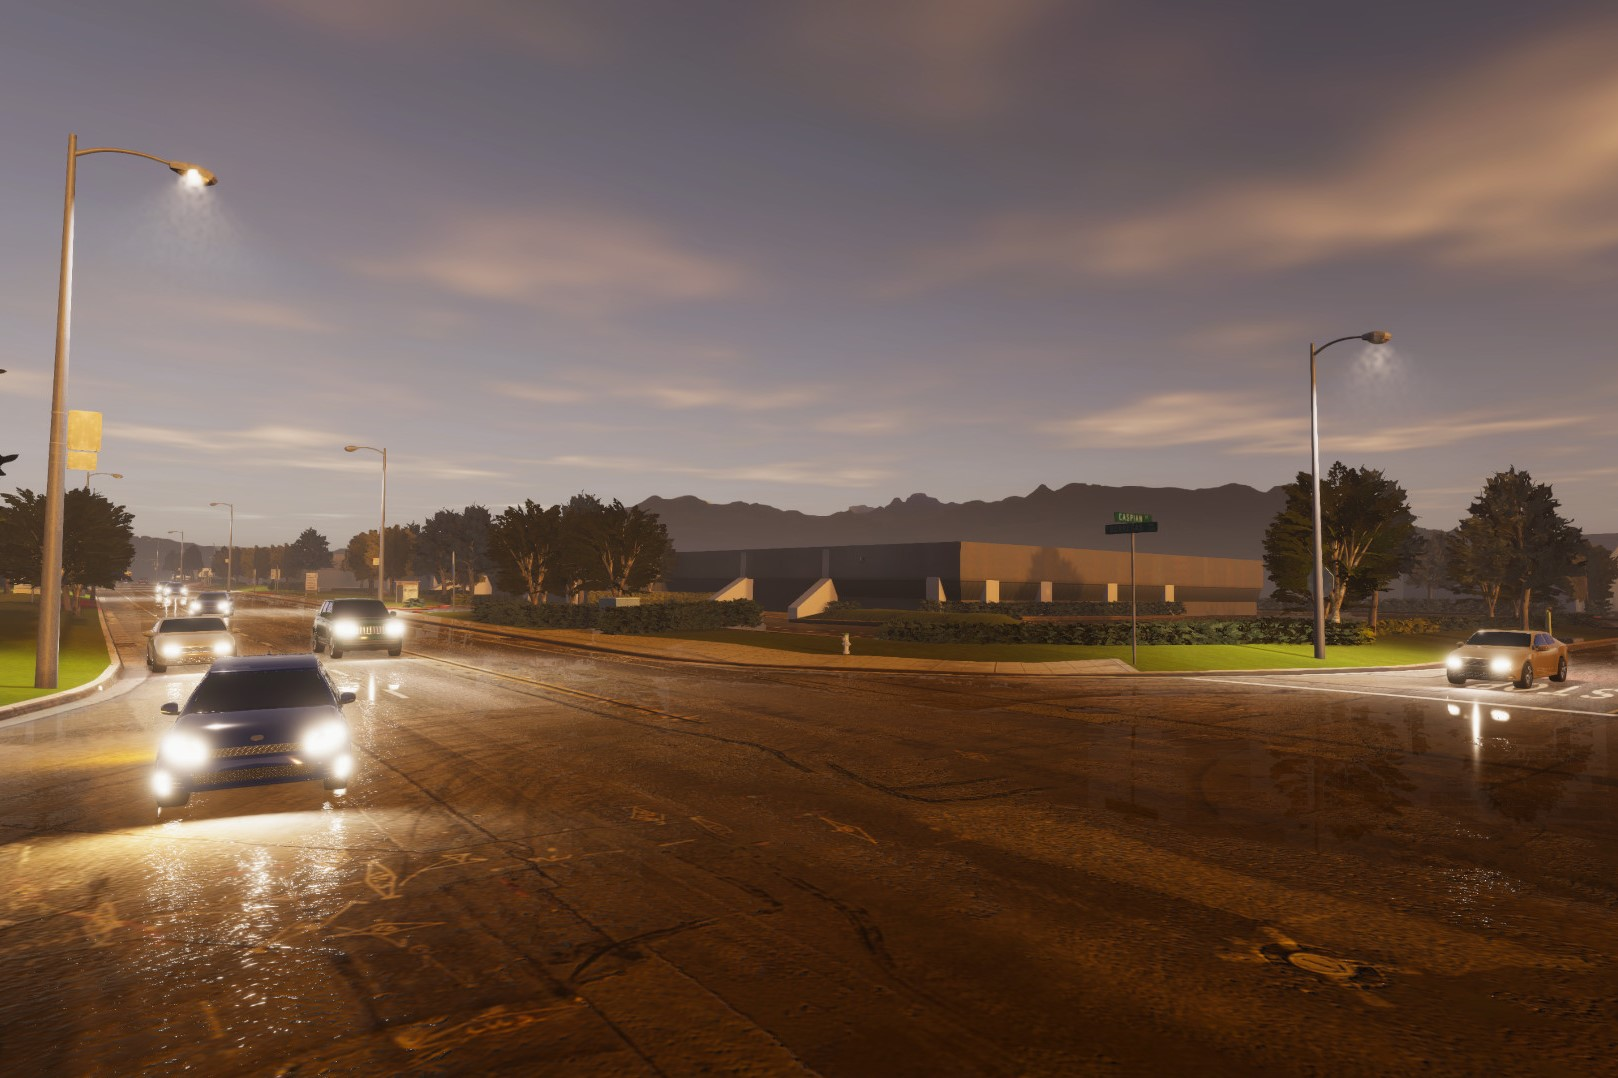
\includegraphics[width=0.5\textwidth]{Simulators/LGSVL.jpg}
    \caption{Source: \url{https://www.lgsvlsimulator.com/about}}
\end{figure}
%https://github.com/lgsvl/simulator

%%%%%%%% Marilou %%%%%%%%%%
\subsection{Marilou}
\textbf{Description:} Marilou is a simulator created by ANYKODE \cite{Marilou_Web}. Marilou is an open map simulator where the user can add objects and hindrances for the robot to navigate around. The simulator is designed to simulate simultaneous localisation and mapping (SLAM) and other localisation techniques. 

\textbf{Open Source:} No (£350)

\textbf{Operating System:} Windows and Linux

\textbf{Game Engine:} Unknown

\textbf{Pros:} Accurately simulates sensors and robot behavior. Easy to add new objects and other controllable entities. 

\textbf{Cons:} As the simulator is not open source, we cannot modify its behavior. Latest release 2018.

\textbf{Conclusion:} Marilou is not a simulator that we can use for this project as it is not open source. In addition, it is not designed with APIs in mind and controlling multiple move able objects at once looks impossible in the current program. 

\begin{figure}[H]
    \centering
    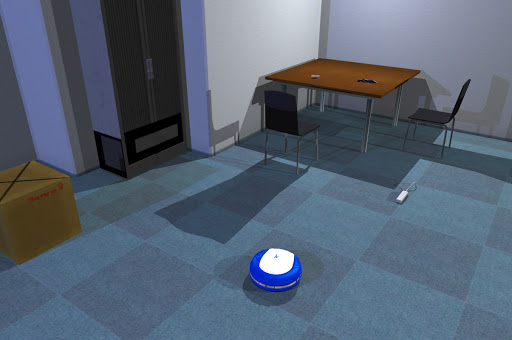
\includegraphics[width=0.5\textwidth]{Simulators/Marilou.jpg}
    \caption{Source: \url{http://www.anykode.com/downloads.php}}
\end{figure}


%%%%%%%% rFpro %%%%%%%%%%
\subsection{rFpro}
\textbf{Description:} rFpro is a driving simulation software which focuses on road-vehicle simulation \cite{rFpro_Web}. rFpro allows for a variety of use cases, from training machine learning models for autonomous driving \cite{rFpro_ML}, to motor racing.

\textbf{Open Source:} No

\textbf{Operating System:} Windows

\textbf{Game Engine:} ISIMotor - A game engine created by Image Space Inc \cite{ISIMotor}. The game engine is used for F1 and other racing games.

\textbf{Pros:} A professionally made simulator that has most of the features we are looking for. Very good graphics and accurate vehicle behavior. 

\textbf{Cons:} rFpro does not give us access to any of the source code. The price is only available upon request, but it is most likely too expensive for this project. 

\textbf{Conclusion:} Even though rFpro contains just about all of the features we are looking for, and is probably the best-looking simulator, it will not work for this project as it is not open source. 

\begin{figure}[H]
    \centering
    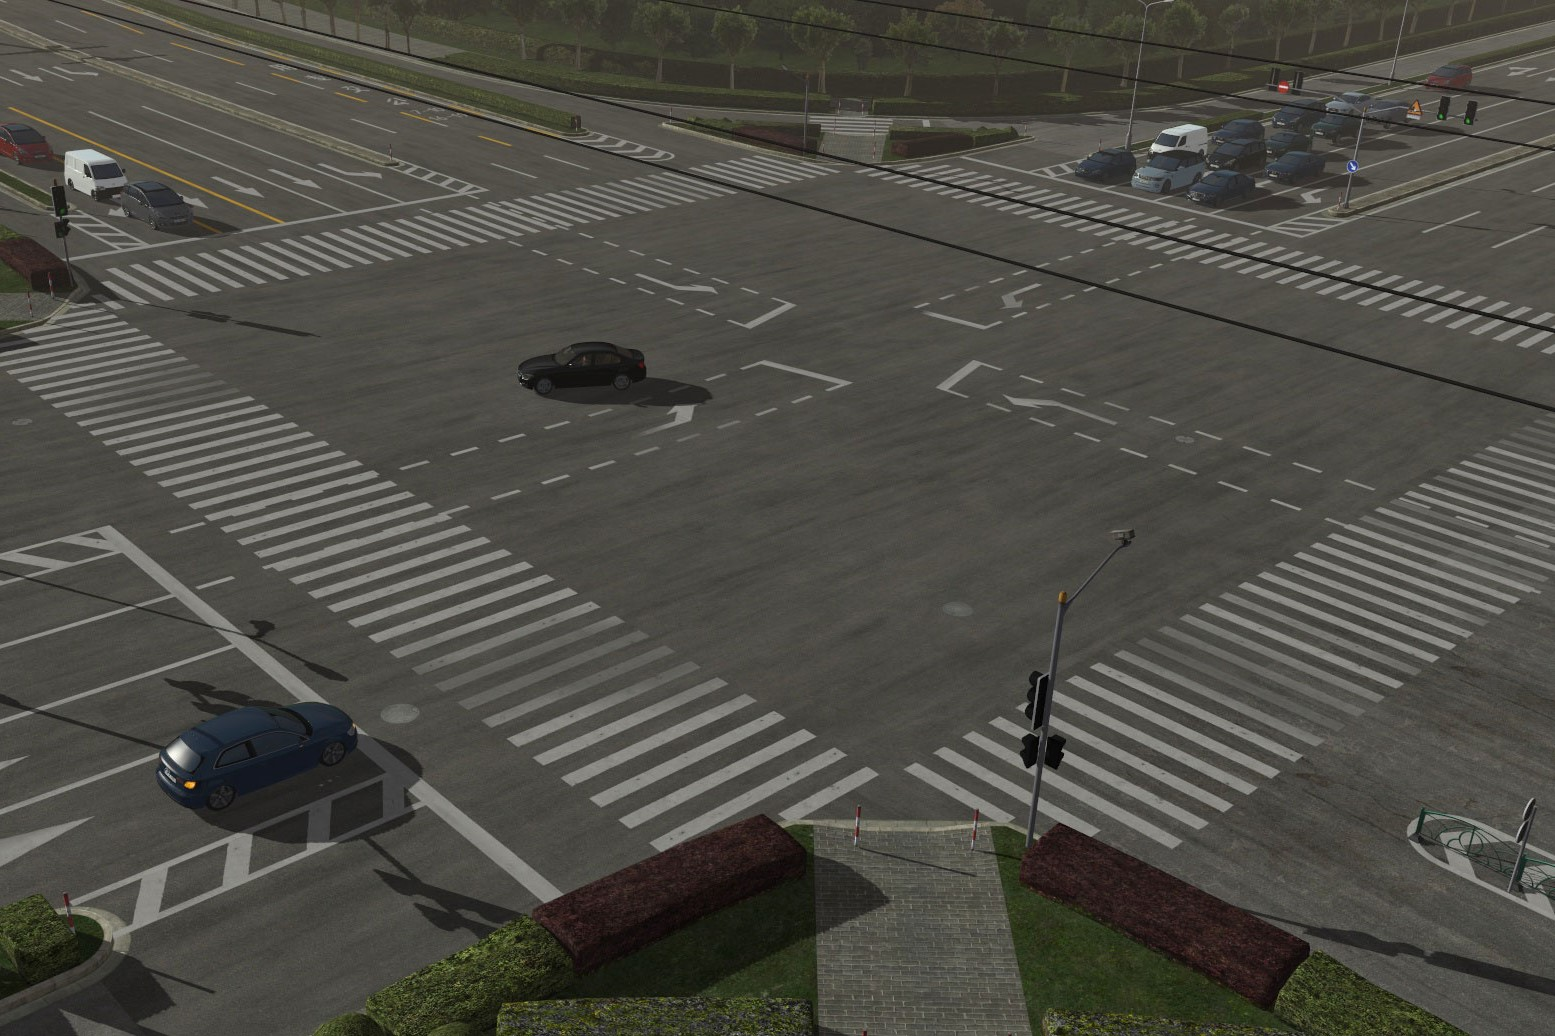
\includegraphics[width=0.5\textwidth]{Simulators/rFpro.jpg}
    \caption{Source: \url{http:https://www.rfpro.com/driving-simulation}}
\end{figure}

%%%%%%%% Rigs of Rods %%%%%%%%%%
\subsection{Rigs of Rods}
\textbf{Description:} Rigs of Rods (RoR) is an open-source physics simulator primarily designed to simulate vehicle physics. The simulator uses soft-body physics which means that if the vehicle collides, its structure will be deformed. This will result in a more accurate simulation.

\textbf{Open Source:} Yes

\textbf{Operating System:} Windows and Linux

\textbf{Game Engine:} Non, creates its own soft-body physics engine

\textbf{Pros:} There is an active community creating modifications for the simulator. Also, the only simulator on the list which uses soft-body physics. 

\textbf{Cons:} There are no APIs currently available. 

\textbf{Conclusion:} As for this project we are not looking for realistic features, but rather certain APIs this simulator will require too much work. It is therefore not a simulator that is worth considering. 

\begin{figure}[H]
    \centering
    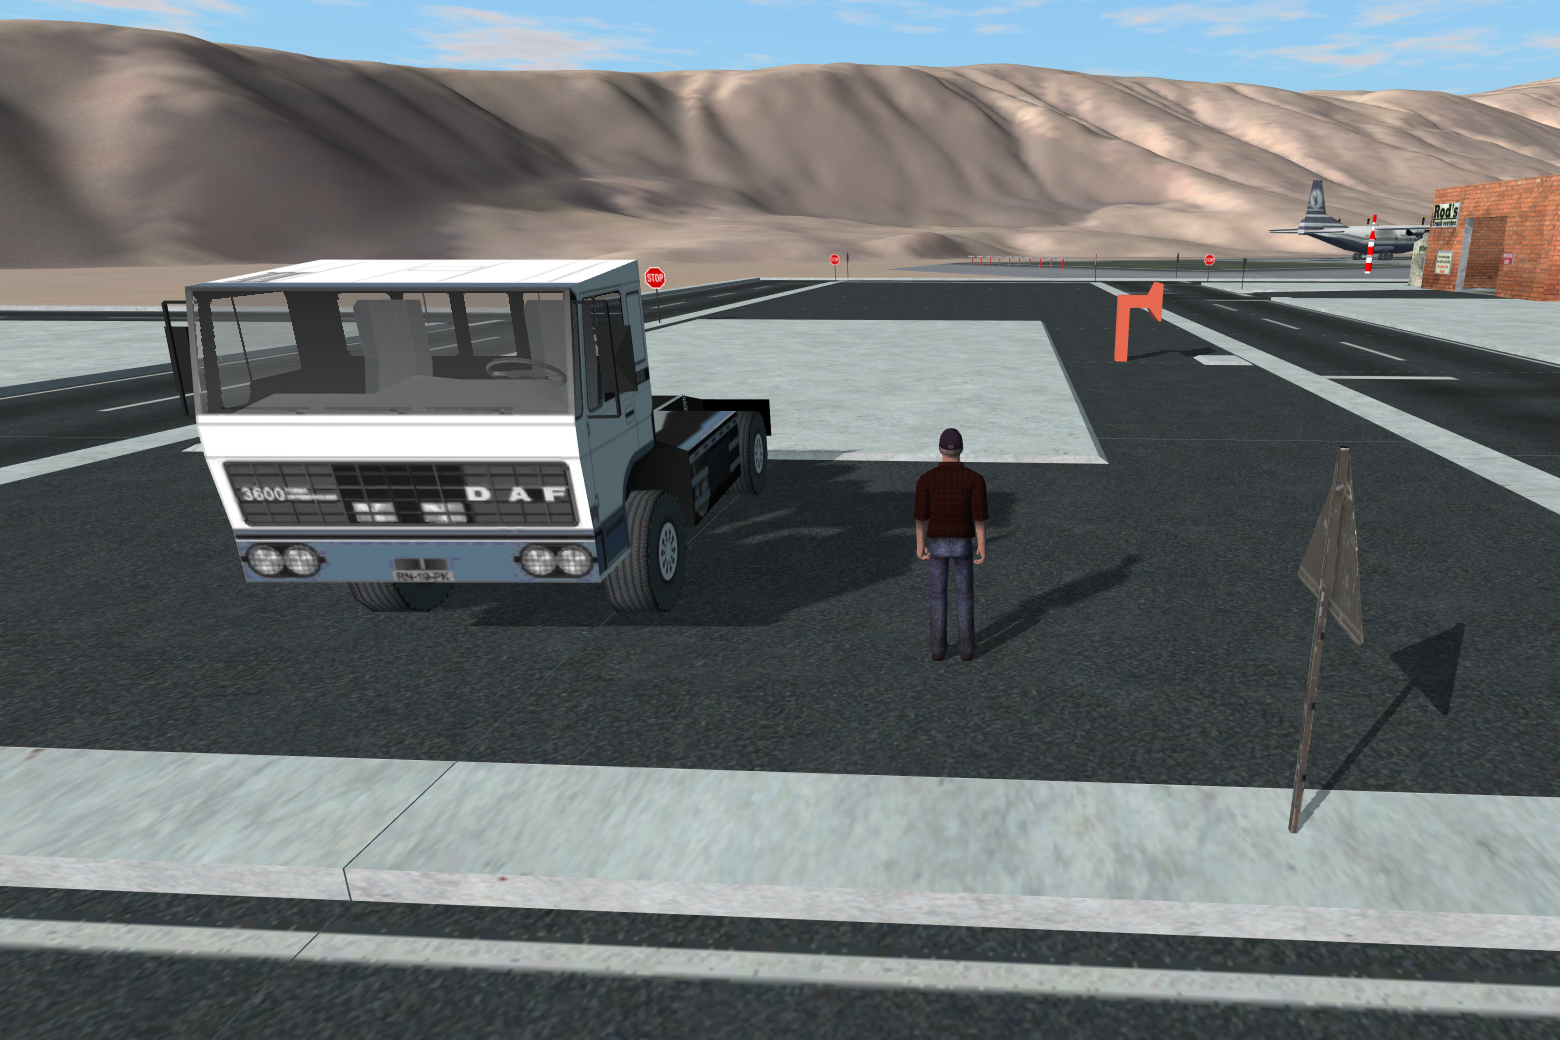
\includegraphics[width=0.5\textwidth]{Simulators/RoR.png}
    \caption{Source: \url{https://docs.rigsofrods.org/gameplay/beginners-guide}}
\end{figure}


%%%%%%%% TORCS - The Open Racing Car Simulator %%%%%%%%%%
\subsection{TORCS - The Open Racing Car Simulator}
\textbf{Description:} TORCS is an open-source racing car simulator. It can be used as an ordinary racing game or as an AI racing research platform. The creators of TORCS used to host competitions on its website among players for who could create the best artificially intelligent racing car \cite{TORCS_Racing}. 

\textbf{Open Source:} Yes

\textbf{Operating System:} Linux and Windows

\textbf{Game Engine:} Non, implemented from scratch.

\textbf{Pros:} Easy to add and create new content. 

\textbf{Cons:} Latest release 2016 but mainly developed in 2008. Also, has no available APIs and no pedestrians.

\textbf{Conclusion:} This simulator is lacking most of the features we are looking for. It is also quite outdated. TORCS is therefore not worth considering. 

\begin{figure}[H]
    \centering
    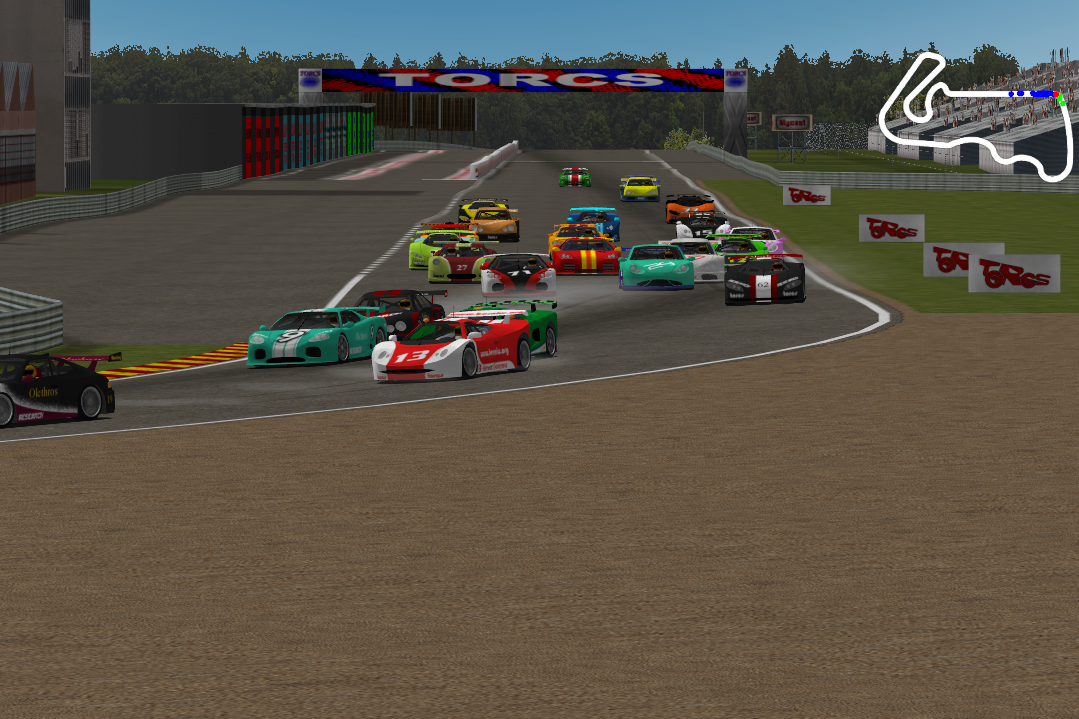
\includegraphics[width=0.5\textwidth]{Simulators/TORCS.png}
    \caption{Source: \url{https://sourceforge.net/projects/torcs}}
\end{figure}

%%%%%%%% Webots %%%%%%%%%%
\subsection{Webots}
\textbf{Description:} test

\textbf{Open Source:}

\textbf{Operating System:}

\textbf{Game Engine:}

\textbf{Pros:}

\textbf{Cons:}


\subsection{Conclusion?}
%https://www.hisour.com/robotics-simulator-42971/


\section{Analysis of Competing Products} \label{AoCP}
In this section, we will look at which of the three simulators to use from Section~\ref{BackgroundLit}.%, as well as 

\subsection{AirSim vs Carla vs Gazebo}
For this section, I started off building the different simulators from source. The aim was to build the simulators in Ubuntu, but due to my outdated graphics card, I was unable to build Unreal Engine. I was however able to run Unreal Engine on Windows by downloading the binary distribution. 
\\~\\
\textbf{AirSim:} The AirSim plugin built successfully on Windows\footnote{\url{https://microsoft.github.io/AirSim/build_windows}}, and I was able to use it in Unreal Engine. The only minor inconvenience was that the simulator has to be built using the Visual Studio 2019 development terminal. However, after installing Visual Studio 2017 which is used to build Carla, I was no longer able to build AirSim. 
\\~\\
As AirSim is built using a game engine, it would hopefully mean it is an easier environment to set up missing features. AirSim is also designed to simulate traffic, unlike Gazebo which is designed for a variety of simulations. 
\\~\\
\textbf{Carla:} Carla built successfully on Ubuntu following this guide\footnote{\url{https://carla.readthedocs.io/en/latest/build_linux}} and after doing these alterations:
\begin{itemize}
    \item As I was using Ubuntu 20.04 I had to install Python2/Pip2 using curl
\item Clang-8 was outdated so I installed Clang
\item Clang-Tools-8 was outdated so I installed Clang-Tools
\item lld-8 was outdated so I installed lld
\end{itemize}
However, as Unreal Engine did not build on Ubuntu I was unable to proceed from here and instead tried on Windows. Carla claims to work on Windows, but I ran into a build error which I was unable to resolve. This seems to be a known issue, and as of the time of writing, is still an unresolved issue on GitHub\footnote{\url{https://github.com/carla-simulator/carla/issues/3605}}. 
\\~\\
Another issue with Carla was the ability to import custom maps \cite{Carlamap}. Carla requires the map to consist of two layers. The first one being the map structure with buildings and roads, whilst the second one will consist of road rules, such as traffic lights, where the cars are allowed to drive, pedestrian crossings, and so on. RoadRunner\footnote{\url{https://uk.mathworks.com/products/roadrunner.html}} can be used to import maps, but this is not a free product.
\\~\\
\textbf{Gazebo:} Gazebo built successfully on Ubuntu\footnote{\url{http://gazebosim.org/tutorials?tut=install_ubuntu&cat=install}}.
\\~\\
Gazebo has all the sensing features we are looking for \cite{Rosique2019}, such as GPS, LiDAR, RADAR, and Ultrasonic. One main drawback with Gazebo is the lack of existing APIs to interact with multiple entities at once. Even though the Gazebo platform has a lot of features, it is not as rich as Unreal Engine \cite{EbeidEmad2018AsoO}. 
\\~\\

\textbf{Conclusion:} As we are not able to build Carla, as well as it being very difficult to change maps, we will discard that one and look at comparing AirSim and Gazebo. 
\begin{itemize}
    \item AirSim and Unreal Engine is more feature-rich than Gazebo. Using Unreal Engine will also minimise chances of finding out something is not possible later on.
    \item Both have the ability to import maps quite easily
    \item Both have the ability to train machine learning models.
    \item AirSim has GPS and Lidar, but it is not clear if it has Ultrasonic or not. Gazebo has more sensing APIs in any case.
    \item Having multiple entities seems easier in AirSim than in Gazebo. 
    \item AirSim is designed for vehicles, whilst Gazebo is designed to be a more generic robotics platform. 
    \item Gazebo is more commonly used than AirSim. 
\end{itemize}
After looking at the information above we have chosen to go with AirSim for this project. This is because AirSim is a plugin for Unreal Engine and that gives us the option to extend the program to anything Unreal Engine allows us to do. 



\chapter{Implementation}
\section{Current Work}
This section will describe what implementation work has been done thus far, and what work that will be done in the near future.
\subsection{AirSim}
AirSim is missing pedestrians, and this has been the first and main priority for the time being. The plan is to add pedestrians in such a way that it will be easily to add cyclists and other mobile robots soon after that. As can be seen in the timeline (Section~\ref{timeline}) this is expected to take roughly 3 weeks. This is also due to the fact that other commitments have been pushed back slightly due to this Interim Report. In AirSim currently we have got a character added, but the character does not yet have any ability to be spawned in or controlled.
\\~\\
AirSim has a lot of available APIs, and the hope is to either incorporate them, or follow their specification when implementing our own. AirSim has a lot of documentation to help with this. There is also an active community where developers can go and ask questions. 
\\~\\
AirSim is built using both Unreal Engine but also Unity. For the time being the plan is to only use Unreal Engine. This is to prioritise rapid development rather than cross game engine debugging. 
\\~\\
An advantage of using AirSim that it could later allow us to use drones in the simulation. This is however not something that will be looked at yet and will be ignored for the time being. 

\subsection{StreetMap}
As mentioned before, the main advantage of using AirSim is that it works as a plugin. This means that we can load any map into Unreal Engine then drive around it. This is what StreetMap allows us to do. Figure~\ref{StreetMapIMG} shows the area around the South Kensington Campus loaded into Unreal Engine with the AirSim plugin also added. The roads are coloured green just to make them easily distinguishable from the ground and the buildings. 
\\~\\
Currently I am looking at ways of updating and improving certain parts of the map. As can be seen in Figure~\ref{StreetMapIMG}, Exhibition road and the Royal Albert Hall are missing. The vehicle can drive off the road, so it is not very important to have that part working however.
\\~\\
Another thing that has to be fixed is that currently buildings do not have a collision box. This means that cars can drive straight through them. This should however hopefully be an easy fix as the buildings are showing up on the existing vehicle APIs in AirSim.  

\begin{figure}[H] 
    \centering
    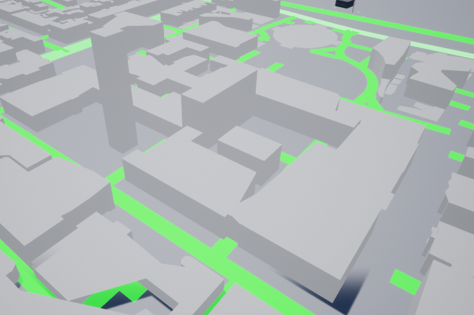
\includegraphics[width=0.5\textwidth]{04_Implementation/Map.png} 
    \caption{Source: Loaded the map of the South Kensington Campus into Unreal Engine}
    \label{StreetMapIMG}
\end{figure}
\section{Future Work} \label{FuturePlanning}
\subsection{Development}
After pedestrians have been added we will need to look at implementing APIs to control them. This should try to follow a similar style to the APIs currently available to control the vehicle. Thereafter we could make minor modifications to the pedestrians so that other mobile robots could be controlled as well. 
\\~\\
The next step would then be to implement the sensing APIs for our new entities. First and foremost, a camera illustrating the pedestrians' point of view would be the most important one,. And once this is done extending it so that it would work for mobile robots as well. 
Following that, we would like to have other kinds of sensors for the mobile robots working. These could for example be ultrasonic and LiDAR. 
\\~\\
When this is done, we will have most of the features we are looking for in the simulator. This will hopefully be done sometime in the middle of March.

\subsection{Evaluation Plan}
Usability
    - Set up simulator
    - Import maps
    - How to run machine learning algorithms on the sim
    - Change vehicle
    - Control pedestrian
    - Use Pedestrian APIs
    
Future work:
    - Depending on what we decide. Could be precision and efficientness. 
Documentation


\pagebreak
\section{Future Timeline} \label{timeline}
\newganttlinktype{rdldr*}{%
  \draw [/pgfgantt/link]
    (\xLeft, \yUpper) --
    (\xLeft + \ganttvalueof{link bulge 1} * \ganttvalueof{x unit},
      \yUpper) --
    ($(\xLeft + \ganttvalueof{link bulge 1} * \ganttvalueof{x unit},
      \yUpper)!%
      \ganttvalueof{link mid}!%
      (\xLeft + \ganttvalueof{link bulge 1} * \ganttvalueof{x unit},
      \yLower)$) --
    ($(\xRight - \ganttvalueof{link bulge 2} * \ganttvalueof{x unit},
      \yUpper)!%
      \ganttvalueof{link mid}!%
      (\xRight - \ganttvalueof{link bulge 2} * \ganttvalueof{x unit},
      \yLower)$) --
    (\xRight - \ganttvalueof{link bulge 2} * \ganttvalueof{x unit},
      \yLower) --
    (\xRight, \yLower);%
}
\ganttset{
  link bulge 1/.link=/pgfgantt/link bulge,
  link bulge 2/.link=/pgfgantt/link bulge}
%------------------------------------------------------------

\ganttset{%
calendar week text={%
\currentweek%
}%
}

\begin{ganttchart}[
hgrid,
vgrid={*{2}{draw=none},dotted,*{4}{draw=none}},
x unit=0.8mm,
time slot format=isodate,
link/.append style={thick},
]{2021-01-01}{2021-06-25}
\gantttitlecalendar{month=shortname, week} \\
% Deliverables
\ganttbar{Interim Report}{2021-01-01}{2021-02-01}
\ganttmilestone{}{2021-02-01}\\
\ganttbar{Final Report}{2021-03-01}{2021-06-09} 
\ganttmilestone{}{2021-06-16}\\
\ganttlink{elem1}{elem2}
\ganttbar{Presentation}{2021-06-07}{2021-06-18}
\ganttmilestone{}{2021-06-21}\\
% AirSim
\ganttgroup{AirSim Development}{2021-01-01}{2021-03-28} \\
\ganttbar{Add Pedestrians}{2021-02-01}{2021-02-14}
\ganttmilestone{}{2021-02-14}\\
\ganttbar{Add APIs to pedestrians}{2021-02-14}{2021-03-17} 
\ganttmilestone{}{2021-03-17}\\
\ganttbar{Evaluation}{2021-03-17}{2021-03-28} 
\ganttmilestone{}{2021-03-28}\\
\ganttlink[link type=rdldr*, link bulge 2=2.5, link mid=.25]{elem8}{elem9}
\ganttlink[link type=rdldr*, link bulge 2=2.5, link mid=.25]{elem10}{elem11}

% Other commitments
\ganttgroup{Other Commtimens}{2021-01-01}{2021-03-28} \\



% Web-App
%\ganttgroup{Web-App}{2021-03-29}{2021-05-30} \\
%\ganttbar{Django Back-end}{2021-03-29}{2021-04-18} \\
%\ganttbar{UI / UX}{2021-04-19}{2021-05-16} \\
%\ganttlink[link bulge=4, link mid=0.5]{elem10}{elem11}
%\ganttbar{REST API}{2021-04-26}{2021-05-16} \\
%\ganttlink[link type=rdldr*, link bulge 1 = 4, link bulge 2=11, link mid=.25]{elem10}{elem12}
%\ganttbar{Deploy App}{2021-05-17}{2021-05-30} 
\end{ganttchart}
\\~\\
When looking at the timeline, it is worth noting that future work might be pushed back if the AirSim development takes longer than anticipated. 
\pagebreak
\section{Extensions}\label{Extensions}
The extensions for the project have not yet be defined, but there are a variety of different options. The current plan is to implement the features required in AirSim and then use them in an extension task. Listed below are some of the suggestions which have been discussed in the supervisor meetings. 
\\~\\
One option would be to try to use the simulator alongside another final year project to simulate the live feed from traffic cameras. There are could several use cases for this. Firstly, it could detect dangerous driving and report it to the police. This could both make people drive more safely as well as making it possible to stop dangerous driving early on. It could also be used to track dangerous traffic junctions to monitor the behavior and detect near-collisions. 
\\~\\
Another option could be to simulate an autonomous wheelchair which exists in the Imperial Robotics Lab. By modeling the wheelchair in AirSim we could try to create an autonomous system and then compare it to the behavior in real life.
\\~\\
A third example could be to try to train a machine learning model for an autonomous robot so that it could navigate around crowded places with cars and pedestrians \cite{ChaoQianwen2015Vifm}. 
\\~\\

\chapter{Ethical, Legal and Safety Considerations}
\section{Ethical Considerations}
As this is just a simulation, there are not really any ethical concerns as such. 
\\~\\
If we however decide to look use the knowledge we learn in our simulator on a physical system there are a few things worth thinking about. Ethical considerations for autonomous systems have been a discussion for a long time \cite{ArkinRonaldC2016EaAS, BorensteinJason2019SCaE}. There are a variety of different ethical concerns. To name just a few, will an autonomous system be responsible enough \cite{BorensteinJason2019SCaE}, who would be responsible for an accident involving a self-driving car, and how could autonomous vehicles impact peoples behavior \cite{moralComputers}. These are not ethical concerns for the project as is, but could become an issue once we decide what the plan for the future is (Section~\ref{FuturePlanning}). 

\section{Legal Considerations}
AirSim has an MIT license which means that we can use the simulator however we like \cite{MITLicense}. This is the same license that is used for StreetMap. In regards to the game engine, as we have chosen to use AirSim which uses Unreal Engine, we are free to distribute the simulator as long as we don't make a gross profit of more than \$1 million \cite{UE5}. 
\\~\\
It could also be worth considering what the UK rules for autonomous vehicles are\footnote{\url{https://assets.publishing.service.gov.uk/government/uploads/system/uploads/attachment_data/file/929352/innovation-is-great-connected-and-automated-vehicles-booklet.pdf}}, if in the future work we decide to introduce a physical system \cite{UKAutoRules, UKAutoRulesGov2}. 


\section{Safety Considerations}
In regards to the project itself, there are no safety issues as it is a simulator being worked on from home. 
\\~\\
As mentioned in the other two sections. If information from the simulator ever gets used in a physical product there are a few things worth considering. Firstly, it is important to remember these are only simulations. Training a machine learning model on the simulator will not accurately reflect the behavior in real life. Secondly, it is important when testing a physical system that it does not for example collide with someone. This could be prevented by driving slowly or not driving where other people or objects might be in the way.


\newpage
\bibliographystyle{IEEEtran} %agsm
\nocite{*}
\bibliography{references}

\end{document}
%%% Local Variables: 
%%% mode: latex
%%% TeX-master: t
%%% End: 
